\begin{Example}[vietnam3]{Student opinion about the Vietnam war}
The revised model, with linear effects of year on each logit,
and with graduate students treated as \pname{yr=7}
 shown in \figref{fig:vietnam3} was fit using
\PROC{CATMOD}.  However, influence diagnostics are
easier to obtain using
\PROC{GENMOD}.
The same model can be fit using \PROC{GENMOD} by defining a dummy variable
for women and an interaction between \pname{yr} and a dummy variable
for men.
\begin{listing}
data vietnam;
   set vietnam;
   yr = year + 2*(year=5);
   mlin =  yr * (sex='M');
   female = (sex='F');
   cell = trim(sex)|| put(year,1.)|| trim(put(response,letter.));
   label yr="Year + 2(Grad)";

proc genmod data=vietnam;
   class year sex response;
   model count = year|sex response|mlin  response|female /
         dist=poisson obstats residuals;
   make 'obstats' out=obstats;
\end{listing}
Normally, one would need to merge the input \Dset\ with the \pname{obstats},
and calculate hat values, Cook's D or other quantities for plotting:
\begin{listing}
%let k=8;
data obstats;
   merge vietnam obstats;
   h = hesswgt * std**2;
   cookd = streschi**2 * h/((1-h) * &k);
\end{listing}
where \pname{k=8} is the number of estimated parameters.

Instead, the \macro{INFLGLIM} (\macref{mac:inflglim}) automates these steps, and
gives various influence plots of residuals from a given
model.  The macro plots all combinations of the variables given
by the \mparm{GY}{INFLGLIM} against the variables given by the \mparm{GX}{INFLGLIM},
using a bubble symbol whose size is proportional to the
\mparm{BUBBLE}{INFLGLIM}, usually Cook's D.

Here, we plot the one-step estimates of change in deviance
($\Delta G_{(-i)}^2$, or \pname{DIFDEV})
due to deleting each cell against hat values,
using bubble symbols with area proportional to Cook's D.
The \mparm{infl}{INFLGLIM} determines the criterion for labeling
potentially influential points.
\begin{listing}
%inflglim(data=vietnam, resp=count,
    class=year sex response,
    model= year|sex  response|mlin  response|female,
    dist=poisson, id=cell,
    infl=%str(difdev>4 or &bubble>1 or hat>1.5*&hcrit),
    gy=difdev, gx=hat, bubble=cookd);
\end{listing}

This plot (\figref{fig:vietgen3}) shows that there are still two
large residuals: 4th year men choose response B substantially less often
than predicted (accounting for over one-third of the model deviance), and first year women choose response C less than
predicted.
%% one figure
\begin{figure}[htb]
  \centering
  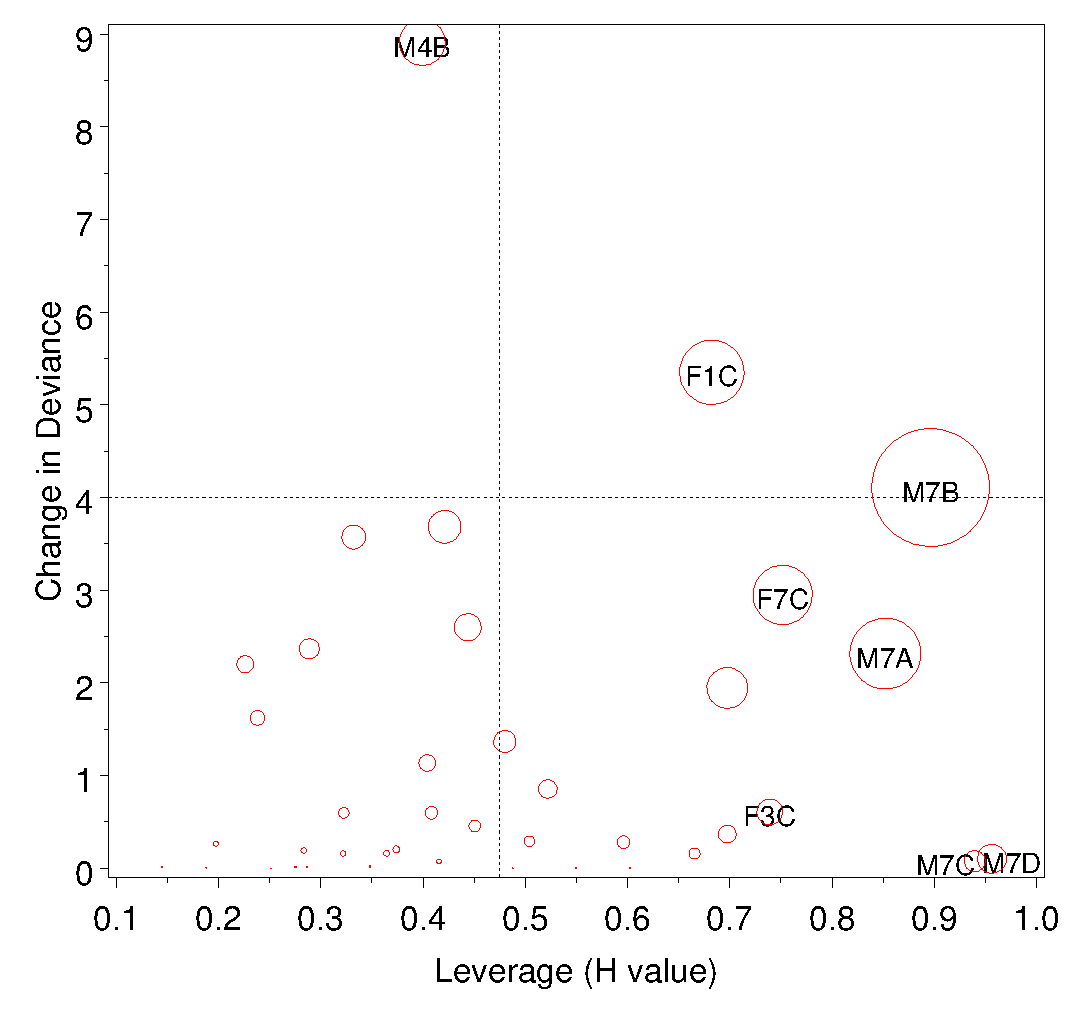
\includegraphics[scale=.6]{vietgen3}
  \caption{Influence plot for model $R = S + Y_{lin}(M)$, Graduate students=7}%
  \label{fig:vietgen3}
\end{figure}
We complete the analysis and this example with a half-normal plot of
these residuals, shown in \figref{fig:vietgen4}.  Although there is
evidence of non-normality in the distribution of residuals,  even the largest
values are within the simulated envelope.
\begin{listing}
%halfnorm(data=vietnam, resp=count,
   class=sex year response,
   model=year|sex  response|mlin  response|female,
   dist=poisson, id=cell);
\end{listing}

\begin{figure}[htb]
  \centering
  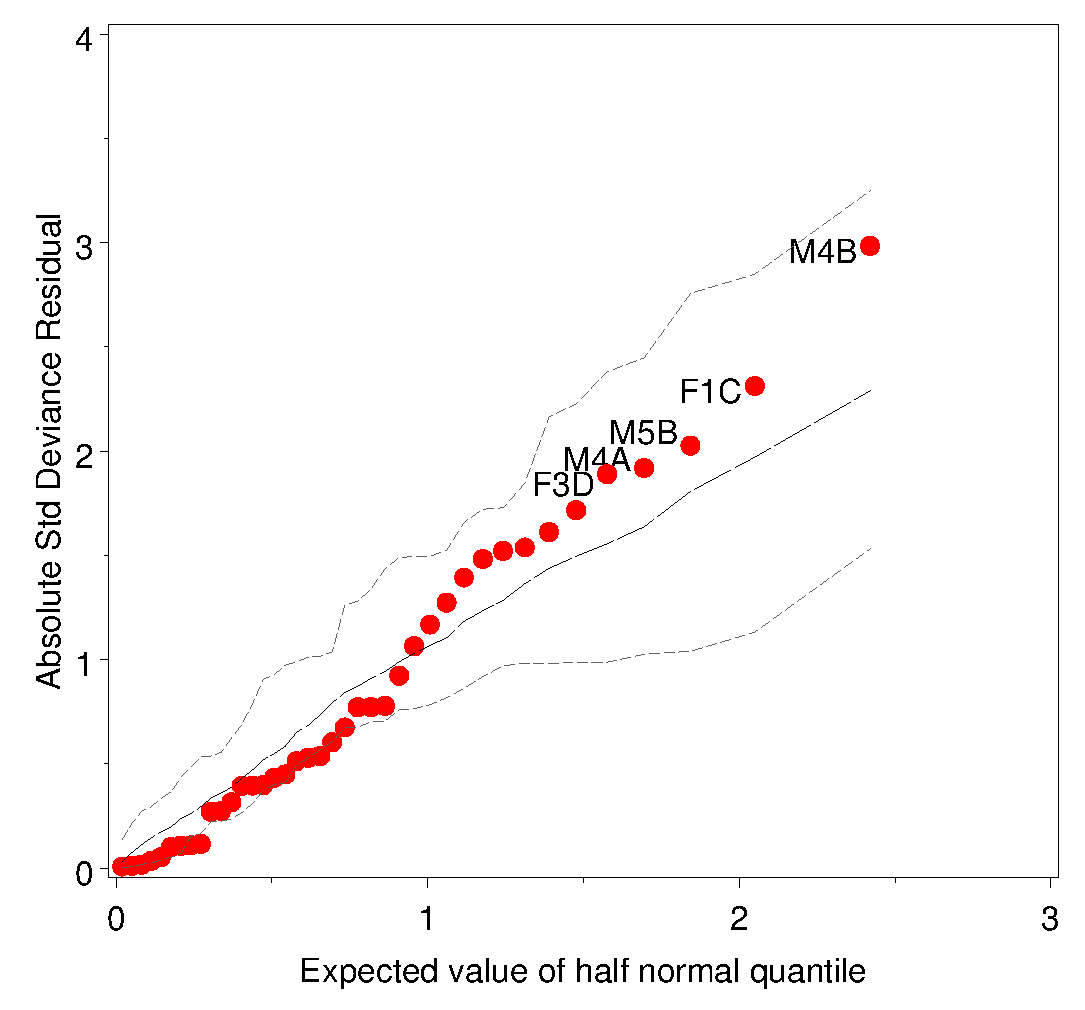
\includegraphics[scale=.6]{vietgen4}
  \caption{Half-normal plot for model $R = S + Y_{lin}(M)$, Graduate students=7}%
  \label{fig:vietgen4}
\end{figure}
\end{Example}
